% 	HTML5 Robot User Interface Project Report: System Architecture
% 	An ASLab Project,
% 	Developed by Daniel Peiró
% 	ETSII, UPM 2014-2015
\chapter{System Architecture} \label{systemarchitecture}
This chapter details the system architecture of HRUI, from three perspectives:
\begin{itemize}
	\item MVC (Model-View-Controller) Architecture.
	\item Client-Server Architecture.
	\item Modular Front-End Architecture.
\end{itemize}
Each of these perspectives correspond to a different software engineering pattern or model. In software engineering, a 
pattern is a generally tried and tested, well documented solution to a particular problem or scenario. Barring very 
specific projects with very specific requirements, it usually is the best solution found to date by the industry, and is 
considered the best practice for it's application. The benefits of using a pattern, instead of developing a completely new 
solution from scratch are many:
\begin{itemize}
	\item Reduces the initial uncertainty of facing a new project, and how to achieve the projects requirements.
	\item Gives a solid foundation for the structure of the program/s that need to be developed, and the purposes each of 
	them serves specifically.
	\item As any best practice, it's likely the most well documented solution to the problem, affording an established 
	knowledge pool to pull from if needed.
	\item Generally, a rigid structure is part of a pattern, which helps consistency and maintainability of the code, since 
	its segmented in a way that keeps its purpose clear and confined.
	\item In large projects, with many developers or teams of developers, it helps breakdown work into different packages, 
	that can be worked on by semi-independent teams (declaring interfaces between components that interact with each other).
\end{itemize}
Several patterns can be applied to a single project, as is the case of HRUI, because of the different sub-systems or 
functional levels of a project. HRUI is a distributed application with a back-end for external controllers and a front-end
with a Graphical User Interface (GUI) for user control. The three architectural perspectives then are:
\begin{itemize}
	\item An overall architecture (MVC Pattern)
	\item A distributed system (Client-Server Pattern)
	\item A front-end subsystem (Modular Pattern)
\end{itemize}
\section{Model-View-Controller Pattern} \label{mvcpattern}
The Model-View-Controller pattern is used in software engineering for systems that require extensive user interaction. It's 
based on three components, each with a very confined set of valid actions and interactions, so that each component doesn't 
overreach in its capabilities. This helps greatly in breaking down tasks, keeping the code close to the business logic, and 
compartmentalizing code by it's particular responsibilities. The three main components of the architecture are, of course:
\begin{itemize}
	\item \textbf{Model}: Holds the "state" of the application. In other words, holds the data that is required for the use 
	of the application.
	\item \textbf{View}: Provides the user with an interface with controllers (and usually a presentation of the model, 
	through requests to controllers).
	\item \textbf{Controller}: Operates on the model, as requested by the view or by other controllers.
\end{itemize}
Of these three components, only the model is generally unique, with several controllers being almost required even in 
smaller projects, and multiple views being useful in some situations.
\begin{figure}[H]
\centering
\captionsetup{justification=centering}
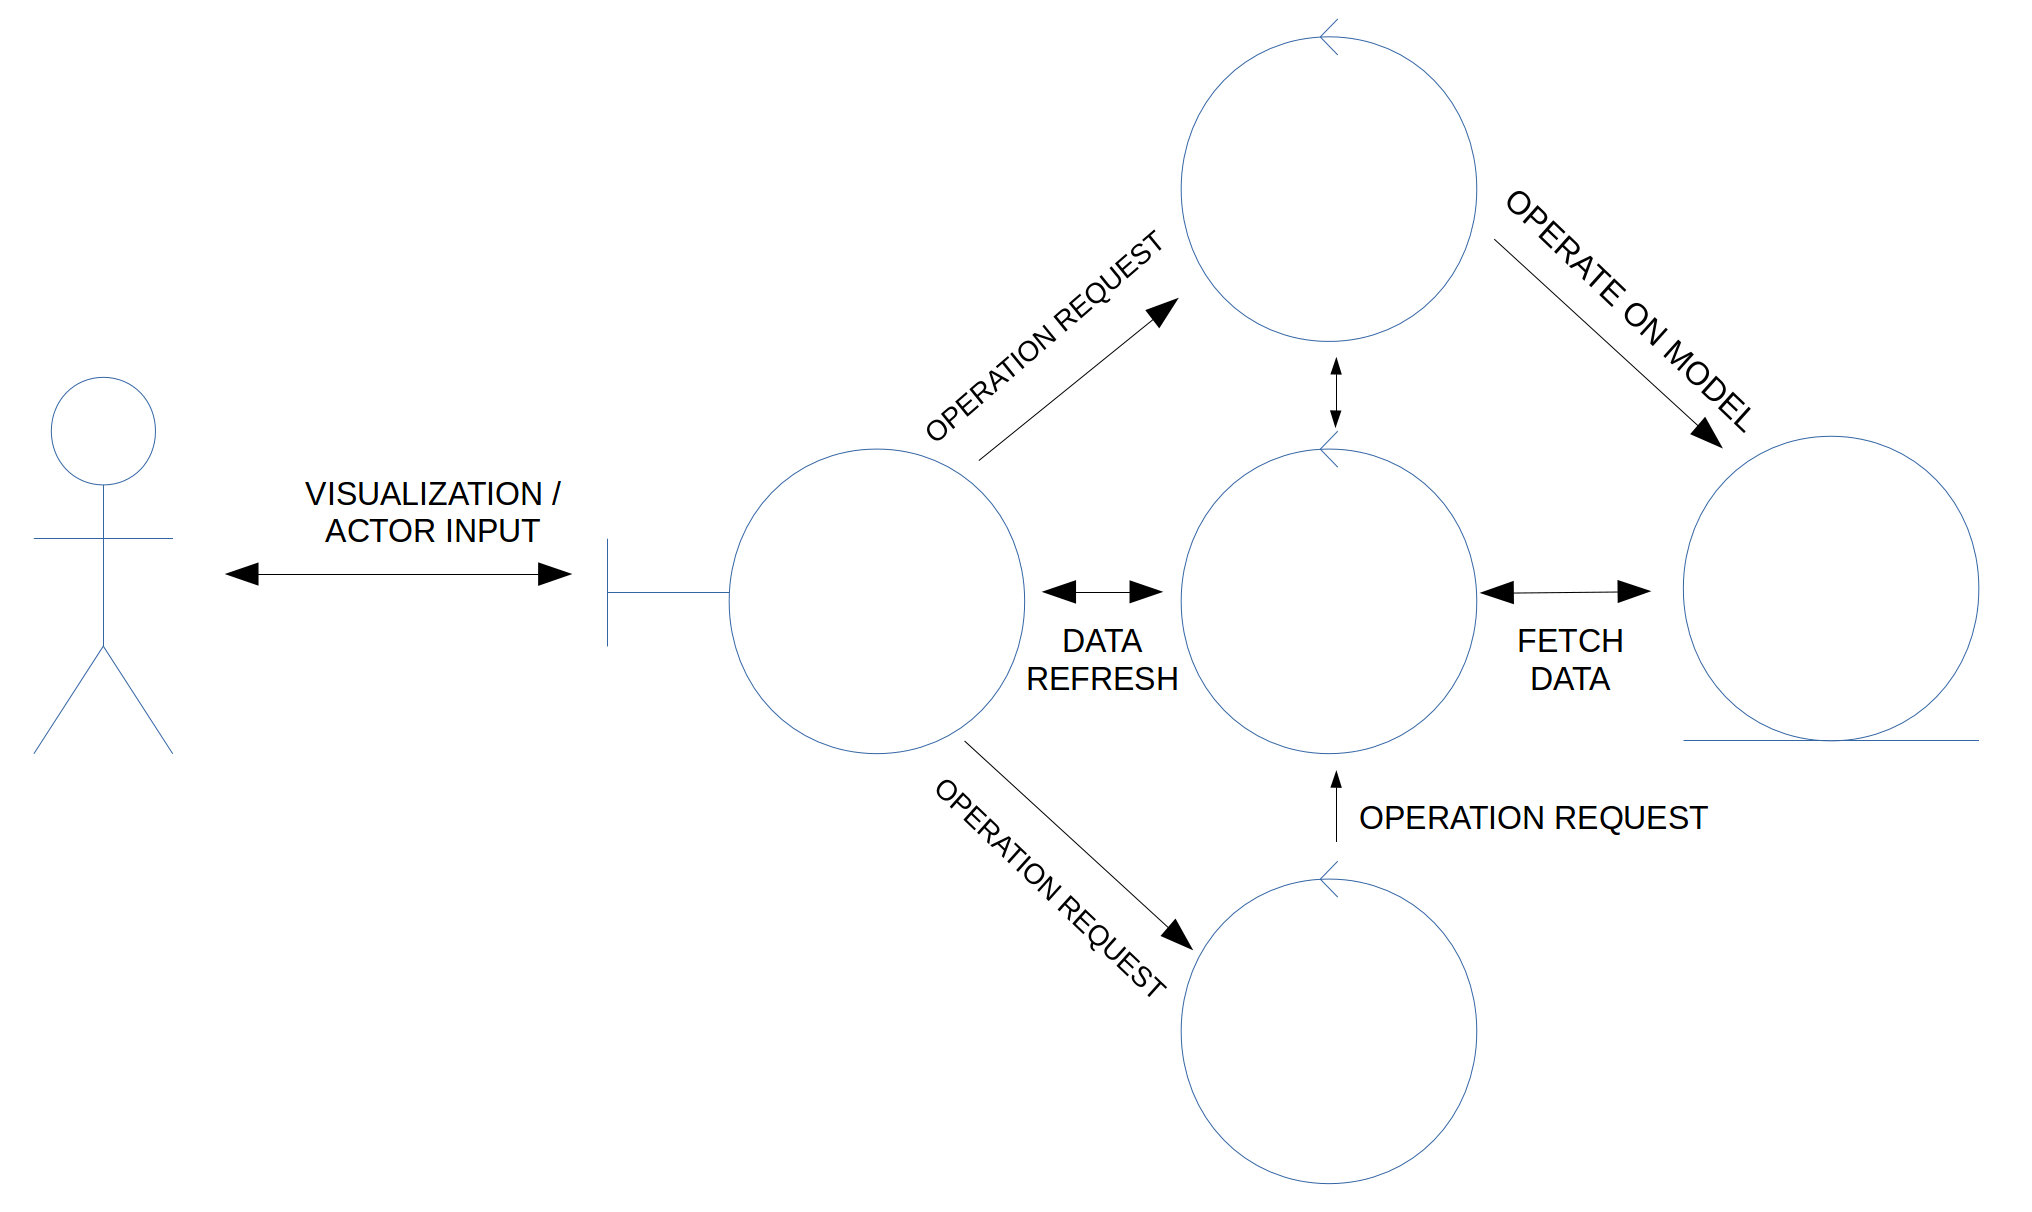
\includegraphics[width=\linewidth]{mvc}
\caption{MVC Architecture UML Diagram}
\end{figure}
In this UML 2.0 (Unified Modeling Language) diagram (robustness analysis diagram, a simplified communication diagram) the 
components are represented as follows (from left to right):
\begin{itemize}
	\item Actor: External agent that uses the system.
	\item Boundary Object: the View component.
	\item Control Objects: the Controller components.
	\item Entity Object: the Model component.
\end{itemize}
This diagram represents how the different components are allowed by the architecture to interact with each other. The View 
can only operate with actors and controllers. Controllers can only operate on the model or other controllers and push data 
to the View. The model can only operate on itself (maintaining the "state" however necessary) and is accessible only to 
controllers. This strict compartmentalization of tasks, allows for very structured applications, that are easy to 
comprehend, maintain and expand upon. Since the actual business logic is contained in controllers, adding logic and 
features to the application becomes as easy as creating a new controller to govern the logic, allocating resources in the 
model to maintain the state, and adding a representation in the view. This breakdown is the true power of the MVC 
architecture, making complex, multi-faceted user interfaces simple to create and expand, while keeping a very simple and 
versatile underlying software structure.\\

HRUI is very well suited to use the MVC pattern. It is essentially a user interface, which requires constant input/output 
to the final user, which is what the MVC pattern was originally envisioned for. But it's also, on the back-end, an 
interface for external robot controllers, and that's where the power of the decoupling between the three components really 
shines in this project. MVC allows for a \textbf{double decoupling} of the application: the separation between how a model 
is represented, and the actual logic that governs the model. In other words, it separates the user experience from the 
programming tasks, both pivoting around the model independently.\\

The user experience is what the View component provides. In this case, the view is an HTML5 web page (which will be 
discussed as a sub-system with an MVC/modular architecture in section \ref{modularfrontendarchitecture}) which grants a 
total decoupling from the host machine, and the back-end as a whole (from this perspective at least, the client-server 
perspective handles that interaction), given this technology's ubiquity. The instructions sent from the View are handled by 
controllers without any knowledge or configuration required by the user. This allows the user to only declare the 
instructions required, without having to process the actual actions. This is the first decoupling.\\

The second decoupling, is that of the model with the actual external robot controllers that need to be programmed for the 
interface to act. The robot programmer or researcher is only aware of the data present in the model at any given time, 
without having to understand anything of how those instructions or data was generated. And most importantly, without having 
to ``care''. For example, the programmer can safely assume that the joystick data present at any time in the model is a 
faithful representation (down to 15 ms accuracy) of the ``state'' of the input. No need to design a user interface, program 
the joystick logic, parse the data through sockets or make an RPC or anything. All the programmer has to do is implement 
his control logic or algorithm, taking inputs and outputs for granted, as they're managed by the integrated controllers. 
This has the enormous advantage of allowing the researcher to do what he's really interested in, programming the robots 
logic, instead of dealing with the work of having to create a user interface.\\

The following diagram, modifies the previous, generic MVC architecture diagram with the particular components of HRUI. It 
does not include all the possible interactions for brevity.\\
\begin{figure}[H]
\caption{HRUI MVC Architecture (see next page)\label{mvcarch}}
\end{figure}
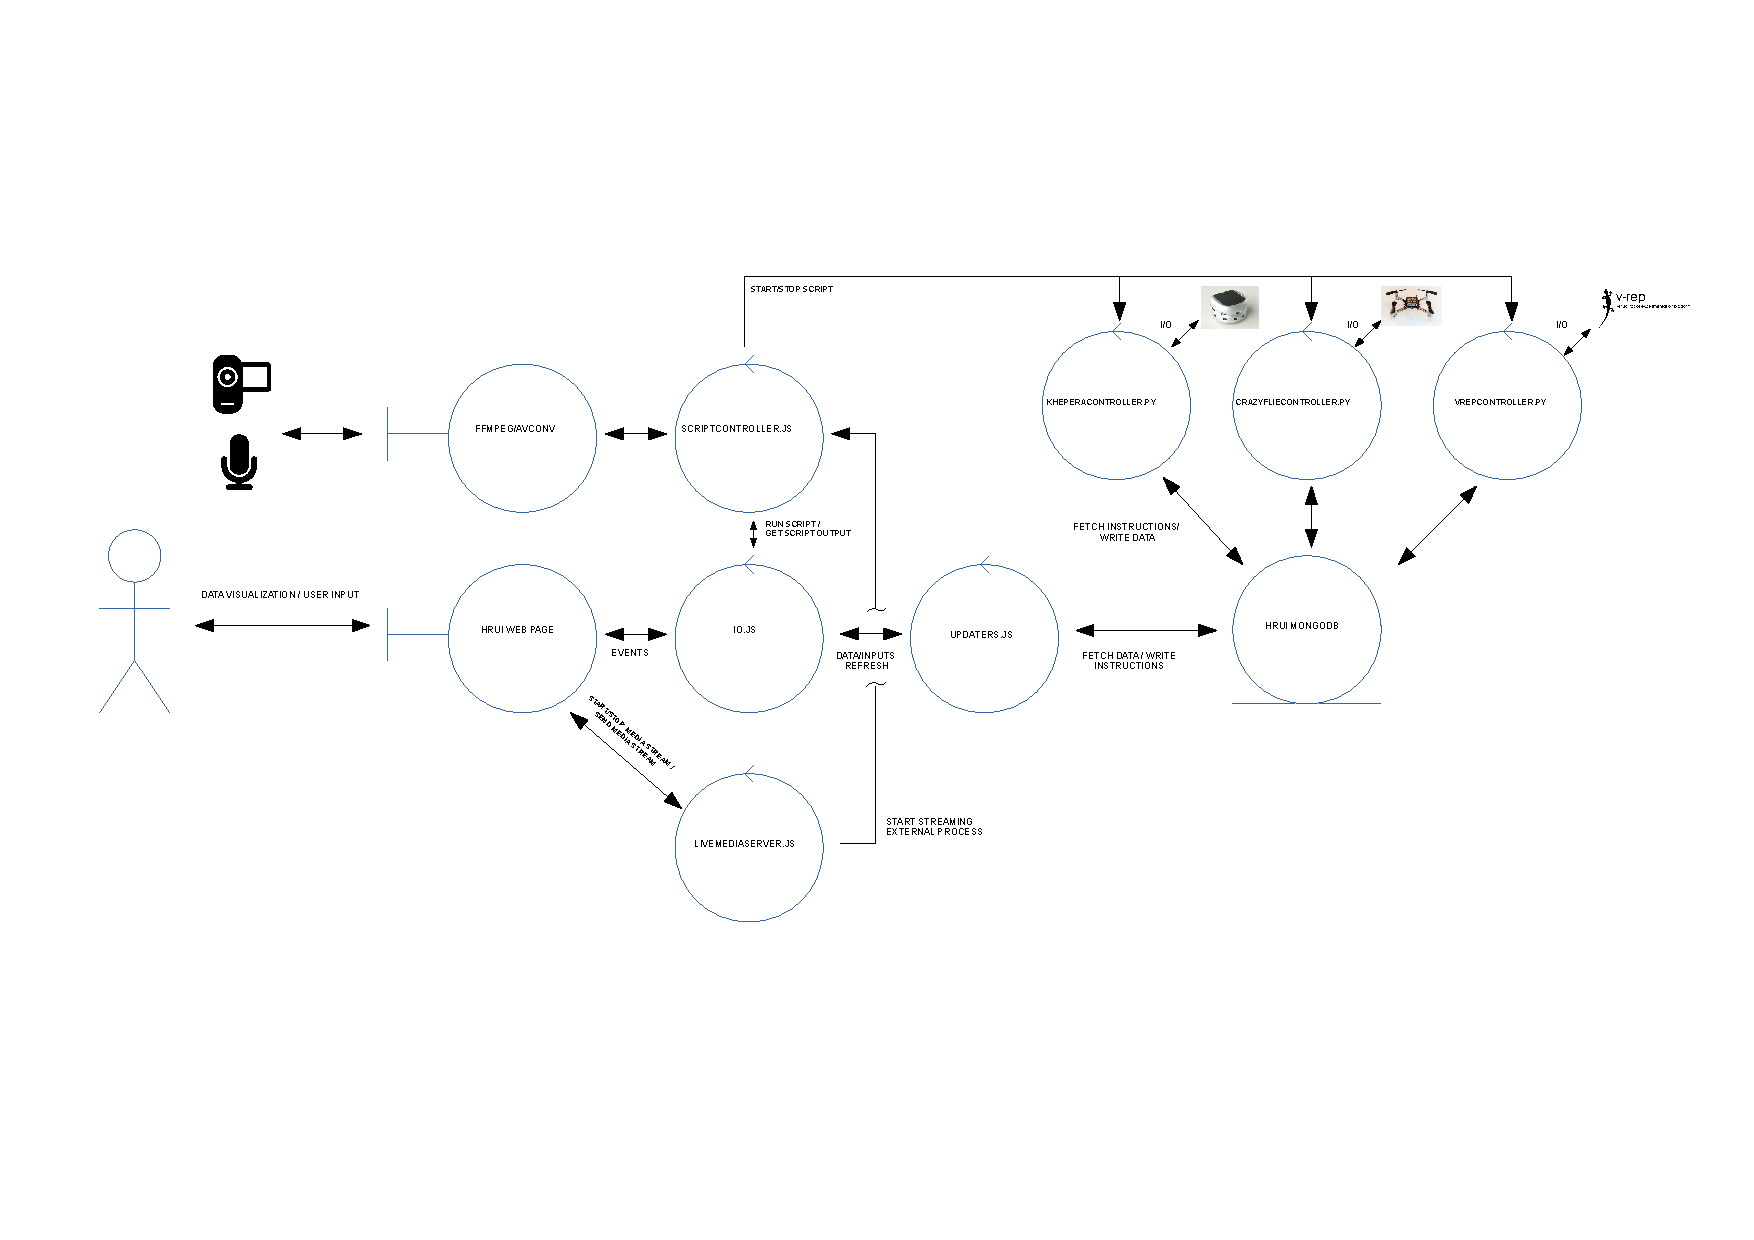
\includepdf[pages={1},landscape]{./img/arch_hrui.pdf}
The following sections briefly describe the structure and functions of each of the components of HRUIs MVC architecture.
\subsection{Model}
The Model component in HRUI is a database that uses the DBMS (DataBase Management System) MongoDB. This technology is 
explained in detail in section \ref{mongodb}, but the main gist is that it's a NoSQL database, making it particularly 
suitable for real-time system r/w requirements and it stores data as documents, which are simply JSON (JavaScript Object 
Notation) formatted objects. In the system architecture, represented in figure \ref{mvcarch}, the Model is the Entity 
object, and can only be accessed directly by control objects, isolating it from the View.\\

HRUIs database has only one collection of documents, called data, in which the state of the application is maintained. It 
initially includes 10 documents, or items, but can be expanded as much as necessary depending on the requirements of each 
robot. Each item must have two properties, for identification purposes:
\begin{itemize}
	\item ``\_id'': An integer value used to identify the item, unequivocally. 0-9 are reserved for the default items.
	\item ``item'': A string that indicates the item's contents.
\end{itemize}
The initial 10 items are:
\begin{itemize}
	\item joystick: holds the state of the primary joystick.
	\item robotData: holds the location, speed, orientation and angular speed of the robot.
	\item robotGeolocation: holds the robots latitude and longitude, and the accuracy in meters.
	\item customDataTest: holds dummy data to test custom data module.
	\item profiles: holds the saved profiles for the profile management module.
	\item mapData: holds a 300x300 binary matrix (0 equals blank, 1 equals obstacle) as a model of the map shown in the 
	data monitor module, which can be used to create a SLAM system.
	\item deviceData: holds the orientation and motion data of the client device.
	\item joystick2: holds the state of the secondary joystick.
	\item voiceCommand: holds the last command registered in the voice command module.
	\item gamepad: holds the state of the gamepad, as registered by the gamepad module.
\end{itemize}
These items hold the basic data required by some of the application modules to function, but the model is in no way limited 
to these items. The programmer can add as many items of any level of complexity as required, for use in different 
controllers or to output to the view through the custom data module, if need be. The same works in the opposite direction, 
the user can add as many inputs as necessary from the View, on the fly, using the custom input module, that can be 
retrieved just as any other item from a controller. This showcases once again the benefits of the MVC pattern, and in the 
case of HRUI the double decoupling of the user interface from the model and likewise with controllers.
\subsection{View}
The View in HRUI is of course the HTML5 web page. The view is considered a sub-system, and has its own architecture, 
described in section \ref{modularfrontendarchitecture}. In the overall MVC architecture, represented in figure \ref{mvcarch}
, the View is the main boundary object, and the only way an actor (in this case the user) can interact with the system, 
thus isolating the actor from the actual procedural logic, and from the model.\\

As each individual module will be discussed in section \ref{modularfrontendarchitecture}, this section only briefly 
explains the overall layout of the UI.\\

The web page, in it's standard format, used in wide screen devices (i.e. Desktops/ Laptops/ Tablets), uses a three column 
layout to present the modules to the user, organized as follows:
\begin{itemize}
	\item \textbf{Left Column. Inputs}: 4 Modules: Primary Joystick, Custom Inputs, Device Orientation and Voice Commands.
	\item \textbf{Center Column. Multimedia}: 3 Modules: Live Video, Live Audio and Geolocation Map.
	\item \textbf{Right Column. Outputs/Utilities}: 4 Modules: Data Monitor, Custom Data, Script Execution (Secondary 
	Joystick is placed here for ergonomic reasons). 
\end{itemize}
This maximizes access to controls when using a multi-touch landscape device, like a tablet, by keeping controls on the 
sides of the page, and the live video stream in the center. The layout is liquid, which means it automatically tries to 
adapt to the viewport (the section of the browser where the page is rendered) and its dimensions dynamically. If the window 
is resized, the layout tries its best to place all different modules in the most readable way, limited obviously by the 
minimum usable size.\\

Using CSS3 media queries (see section \ref{html5styling} for more), the layout changes to a one column design when the page 
is used on a smartphone, or otherwise portrait oriented device. Since it's not possible to represent even a few modules at 
the same time on a small, vertical screen, the layout maximizes the use of one module at a time, allowing the user to 
scroll from one to the other as needed. It also frees up screen real estate by hiding the module selection toolbar in a 
side menu, that can be pulled out and hidden by using the menu button at the top left of the page. This toolbar can also be 
hidden in the desktop version.
\begin{figure}[H]
\centering
\subfloat{{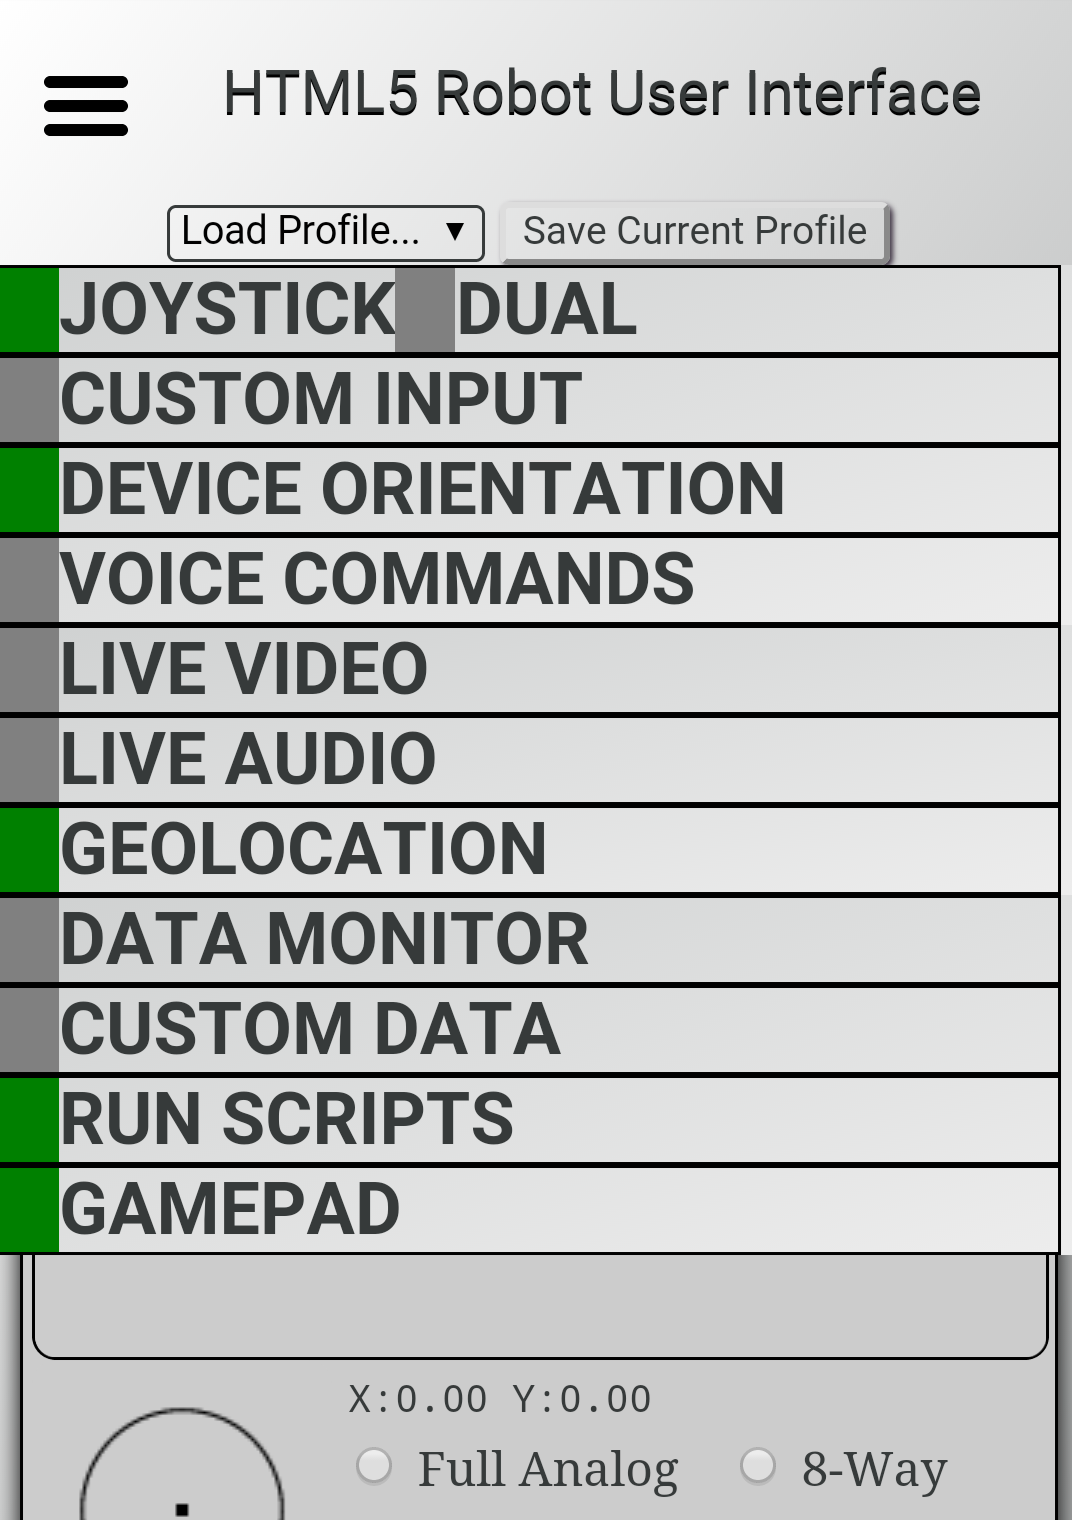
\includegraphics[width=\linewidth/5]{sidebar}}}
\subfloat{{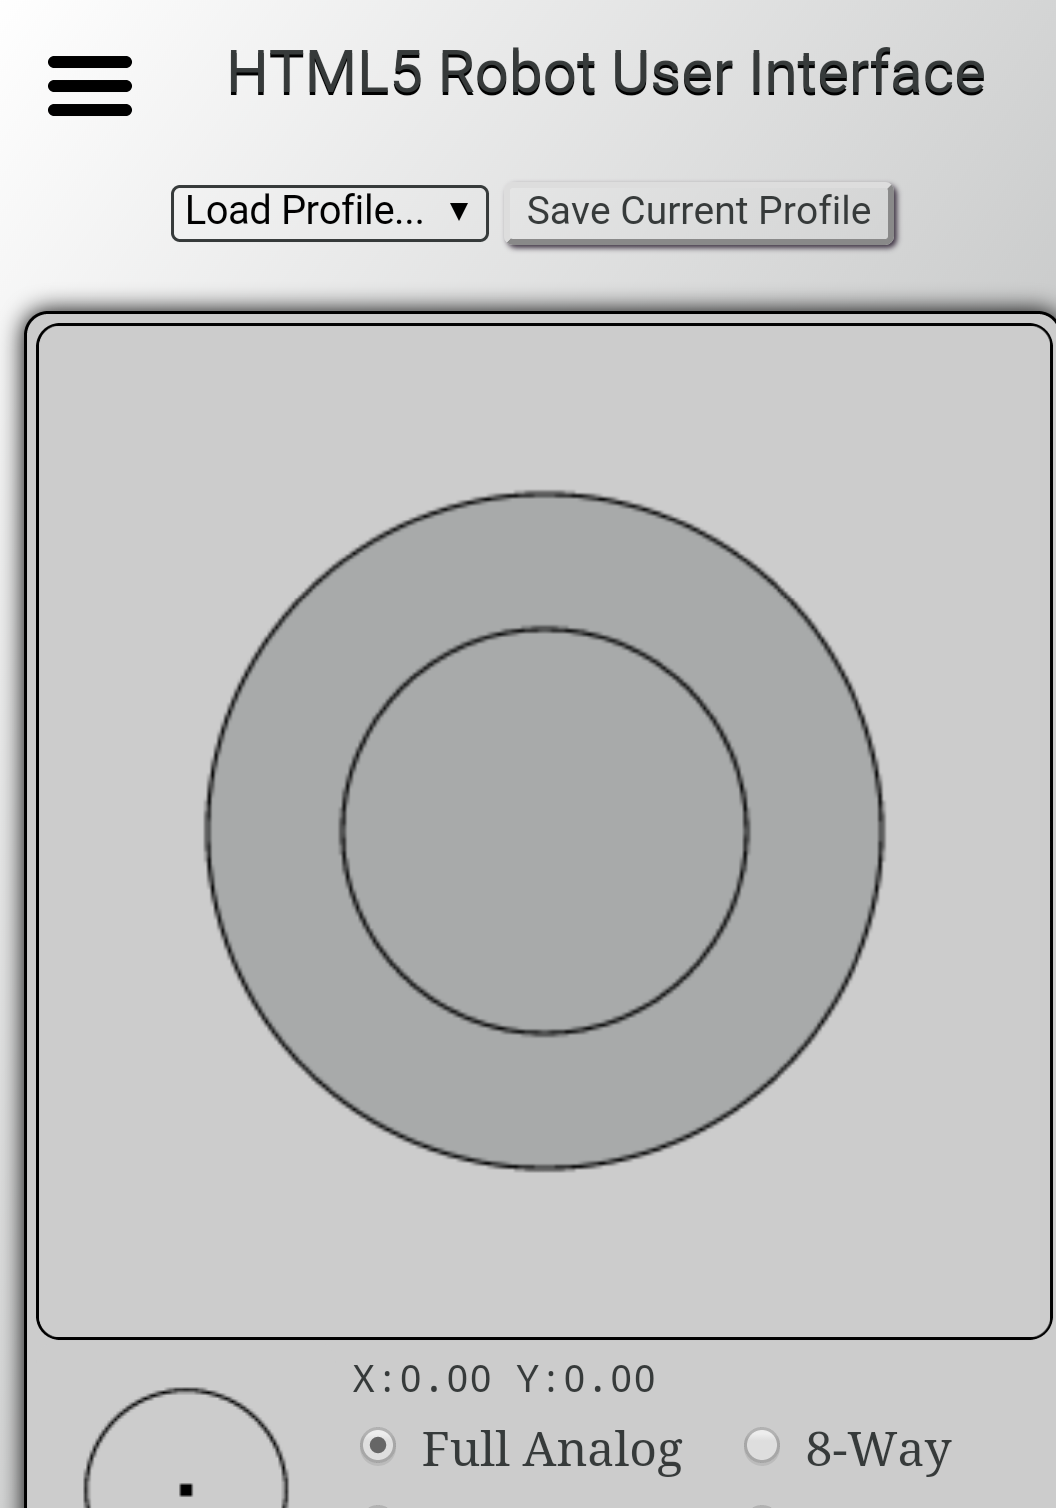
\includegraphics[width=\linewidth/5]{nosidebar}}}
\caption{HRUI Mobile Side Bar}
\end{figure}
\begin{figure}[H]
\centering
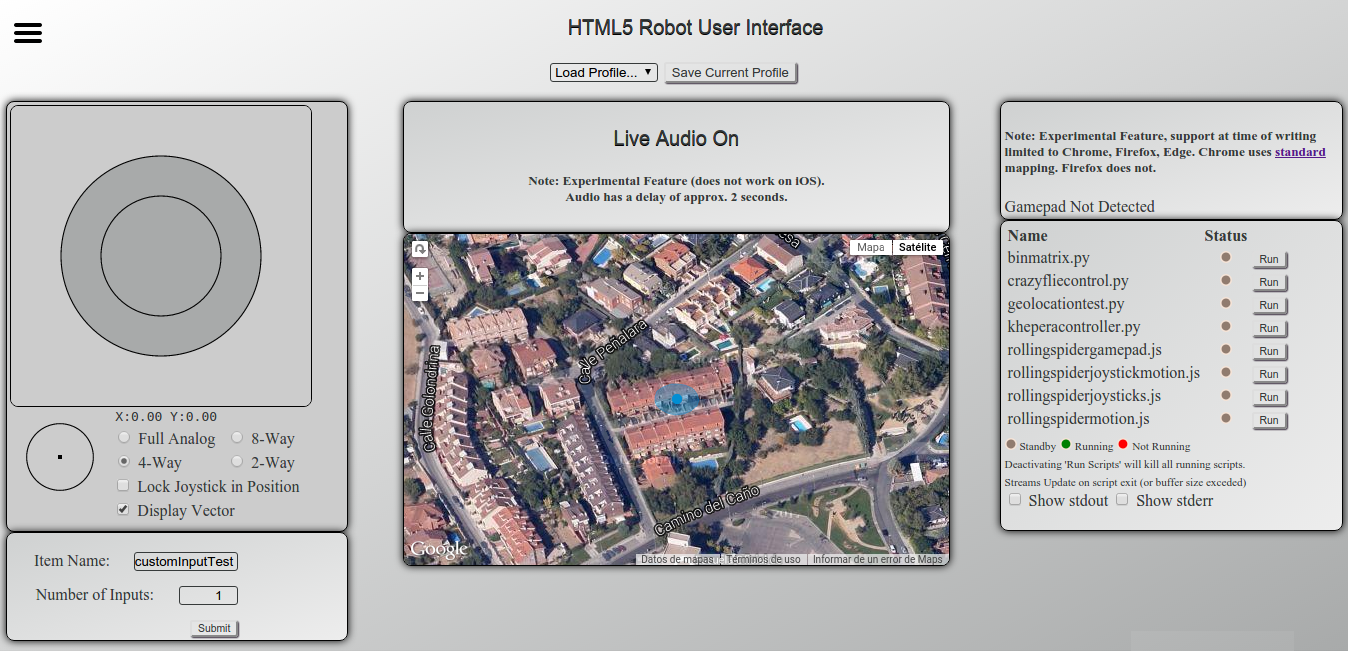
\includegraphics[width=\linewidth]{hrui3column}
\caption{HRUI Desktop/Laptop/Table Three column design (Toolbar hidden)}
\end{figure}
\subsection{Controllers}
HRUI controllers are divided in two distinct categories:
\begin{itemize}
	\item \textbf{Internal Controllers}: They're integrated in the application, controlling the inputs and outputs from the 
	view to the model. In the system architecture (figure \ref{mvcarch}), they are represented between the View and the 
	Model. There are four main internal controller modules: updaters.js, scriptController.js, io.js and liveMediaServer.js.
	\item \textbf{External Controllers}: Designed by the programmer or researcher to input and output data between the 
	model and a robot/s. In the system architecture (figure \ref{mvcarch}), they're represented between the model and the 
	robots. They're not integrated in the application and can only interface with the model and their respective robots 
	directly. As a proof of concept, three external controllers have been developed to control three different robots, all 
	three written in the Python programming language (see section \ref{python}): 
	\begin{itemize}
		\item vrepcontroller.py: controls a virtual Khepera III robot in the robot simulator V-REP (see section 
		\ref{vrepvirtualkheperaiii}).
		\item kheperacontroller.py: controls a Khepera III robot (see section \ref{kheperaIII}).
		\item crazyfliecontroller.py: controls a Crazyflie 2.0 drone (see section \ref{crazyflie2}).
	\end{itemize}
\end{itemize}
\subsubsection{Internal Controllers}
\begin{itemize}
	\item \textbf{updaters.js}: This module is the controller that collects all requests from other controllers to modify 
	or get data in the model and processes them. It's represented in the system architecture (figure \ref{mvcarch}) between 
	io.js and the model. Each of the functions it holds can be considered itself a sub-controller, that is designed to 
	respond to each distinct requests. The power of the MVC architecture allows this code to be reasonably close the 
	business logic, making it easily comprehensible and maintainable. The module exposes an interface to other modules, to 
	call the necessary update to the database as needed. The main consumer of this interface is io.js.	
	\item \textbf{io.js}: Configures the Socket.IO framework (see section \ref{html5websockets}) to capture and send events 
	to and from the View. It's represented in the system architecture between the View and the rest of the controllers (
	except for liveMediaServer.js, that interacts directly with the view for media streaming). The event model will be 
	discussed in section \ref{clientserverpattern} as part of the Client-Server pattern. After initial configuration, this 
	module simply declares ``hooks'' for each event. This means it establishes a handler function (a controller in itself) 
	to process each event. The handler functions are exposed by updaters.js and scriptController.js, to service the request 
	of the View, or other controllers.
	\item \textbf{scriptController.js}: Handles requests from other controllers and from the view to execute or kill 
	external scripts and programs. This includes starting and ending avconv/ffmpeg media stream acquisition and running and 
	killing JavaScript and Python scripts added to the userscripts folder (normally, these will be external controllers, 
	but not necessarily) at the request of the View (through an io.js event hook). Requests to this controller are made by 
	io.js and liveMediaServer.js.
	\item \textbf{liveMediaServer.js}: Configures media stream reception and relay to the View, using raw websockets (see 
	section \ref{html5websockets}).
\end{itemize}
A UML 2.0 Communication/Collaboration diagram for internal controllers is presented in figure \ref{controllerarch}. 3 Use 
cases are presented in the diagram:
\begin{enumerate}
	\item User moves virtual joystick. Triggered by the user through a mouse/touch event.
	\item Periodic update of robot data (position, orientation, velocity and angular velocity).
	\item User turns on Live Video feed.
\end{enumerate}
This diagram uses the following format to represent messages between objects:\\

\centerline{[sequenceNumber.] methodName(parameters) [: returnValue]}
\begin{itemize}
	\item {[}sequenceNumber.{]} : Numbering that indicates the order of messages for each use case.
	\item methodName(parameters) : The ``method'' invoked and the parameters passed. Method is used in the sense of object 
	oriented programming, where any action that an object requests from another is called a method. Parameters are 
	arguments that the invoked action requires.
	\item {[}: returnValue{]} : The response data received after the invocation of the method, if any.
\end{itemize}
\subsubsection{External Controllers}
Since the external controllers depend on how each robot's API is implemented, it's particular inputs and outputs and 
communication method, the UML 2.0 communication diagram presented in figure \ref{extcontrollerarch} is very abstract, 
devolving into a component diagram between the robot and the controller indicating the interface exposed by the robot and 
it's required implementation.
\begin{figure}[H]
\caption{HRUI Internal Controllers Communication Diagram (see next page)\label{controllerarch}}
\end{figure}
\begin{figure}[H]
\caption{HRUI External Controllers Communication Diagram (see next page)\label{extcontrollerarch}}
\end{figure}
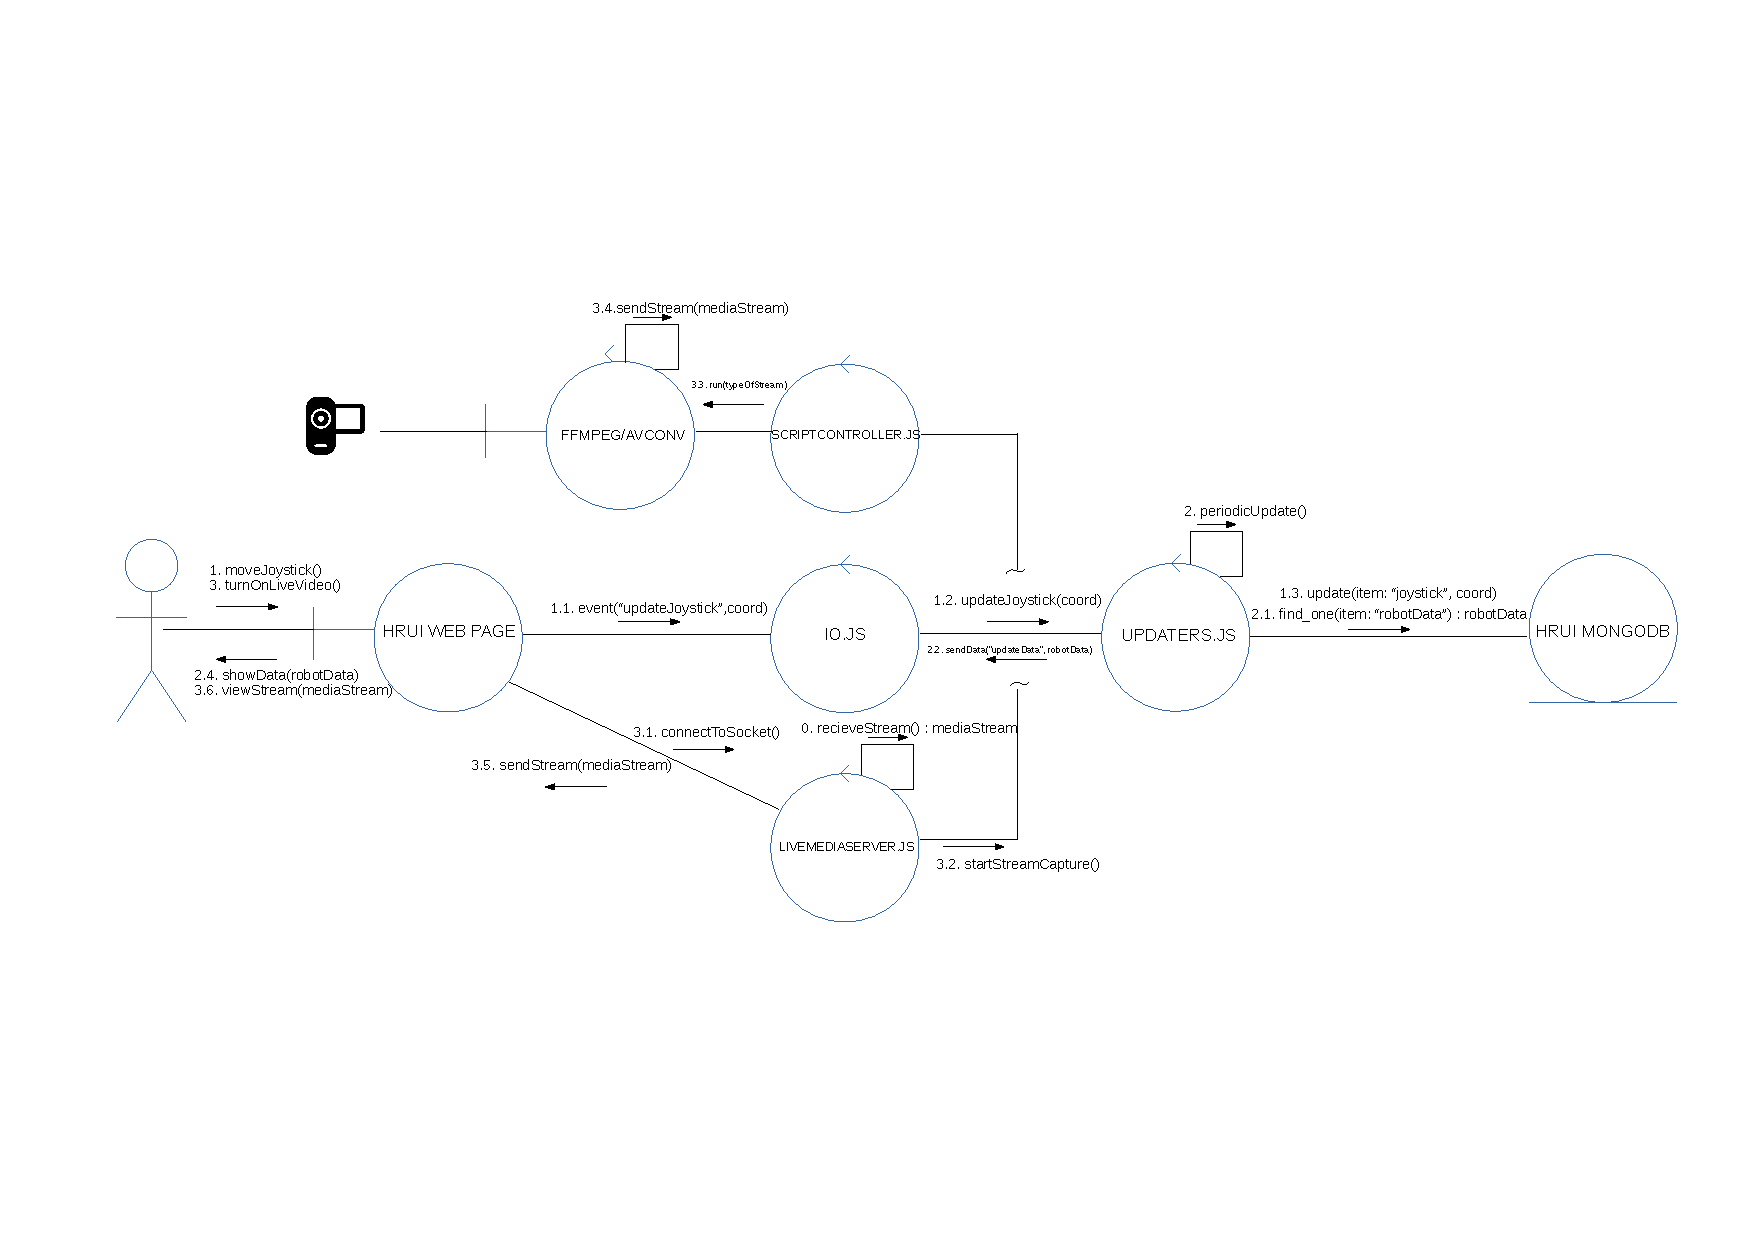
\includepdf[pages={1},landscape]{./img/arch_controllers.pdf}
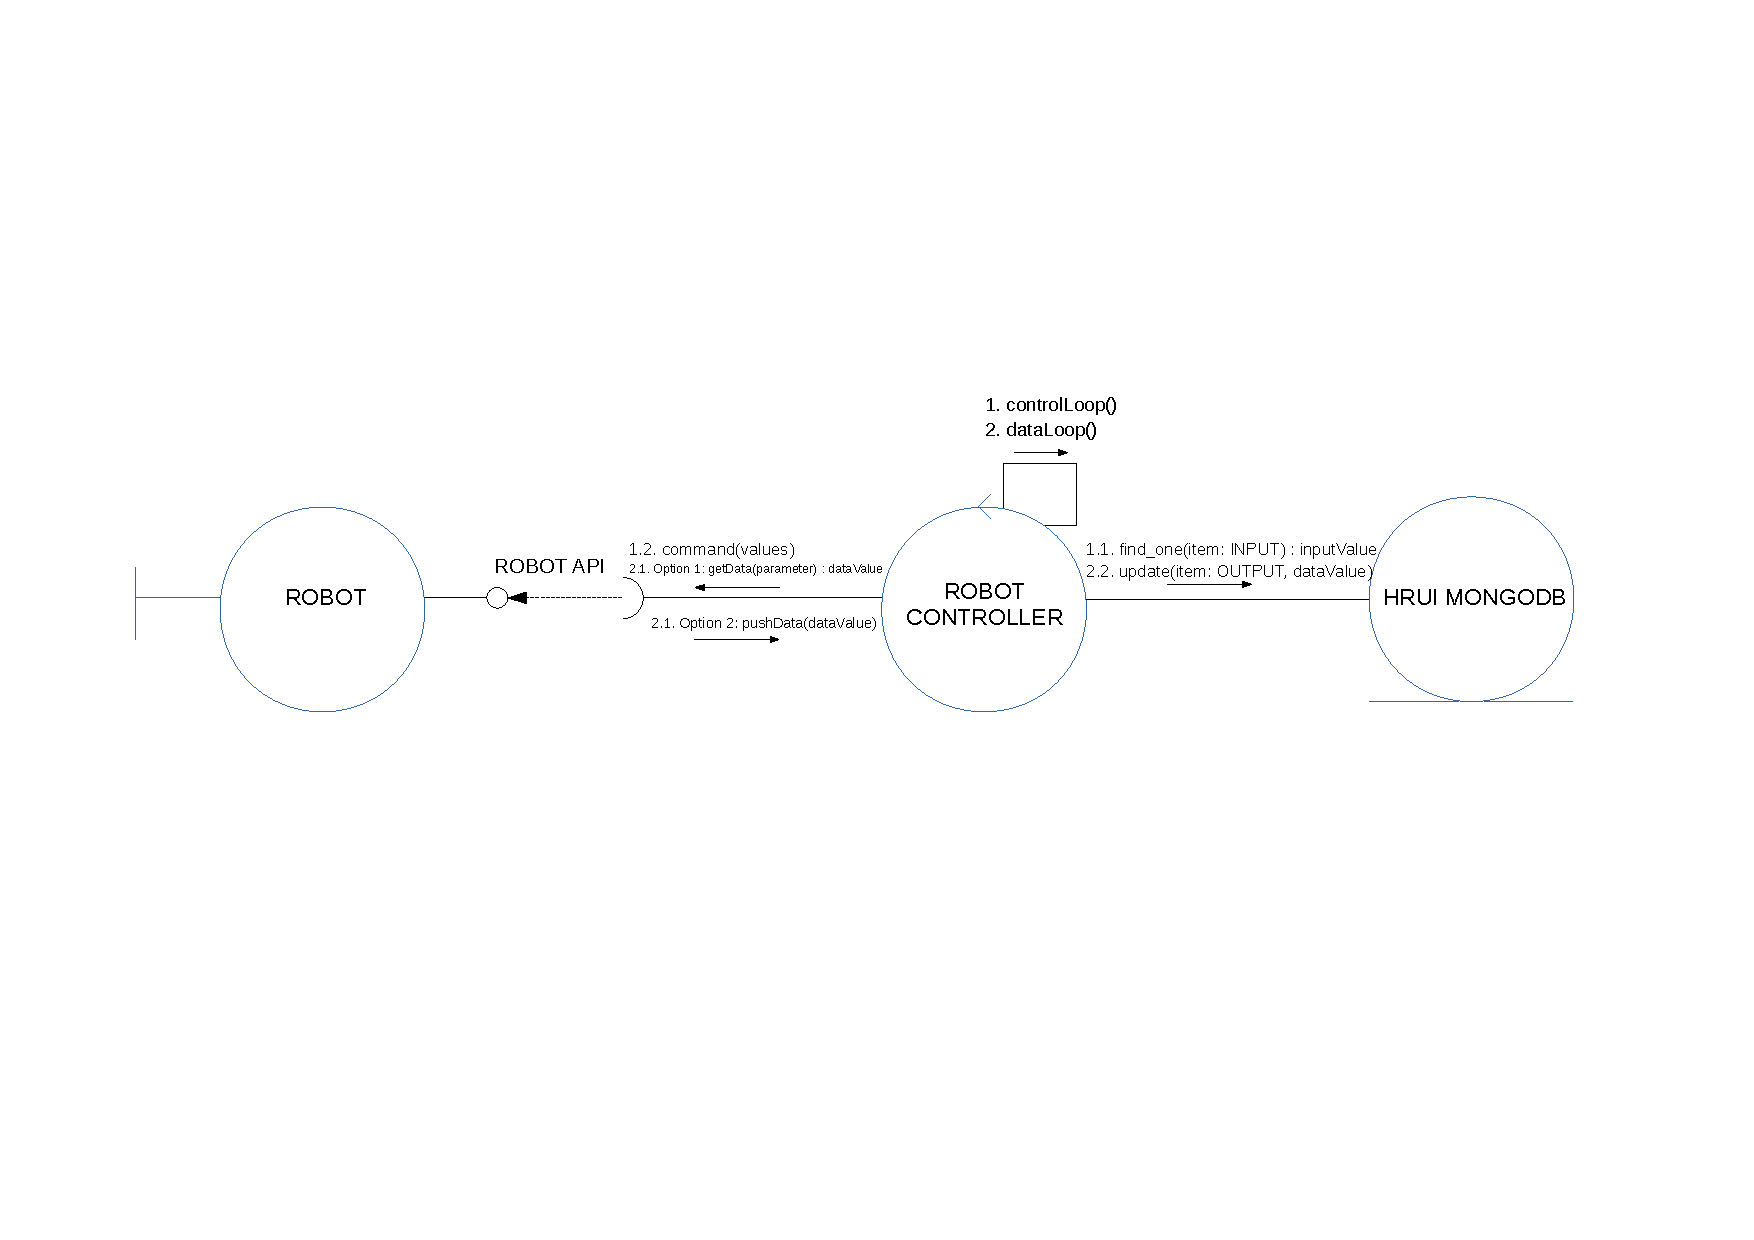
\includepdf[pages={1},landscape]{./img/arch_ext_controllers.pdf}
\section{Client-Server Pattern} \label{clientserverpattern}
The Client Server Pattern is a structure for distributed software (software that is run on different machines pertaining to 
the same system or in order to achieve a common goal or service) that separates components into two main stereotypes:
\begin{itemize}
	\item \textbf{Client}: A component that requests services and resources from a server, and does not provide any of it's 
	own resources to other components. Generally there are multiple clients per application, although this is not a 
	requirement.
	\item \textbf{Server}: A component whose purpose is to provide services and resources to clients. Typically there is only 
	one server component, although this server itself can be a distributed system across many machines that relate to each 
	other using the same client-server pattern.
\end{itemize}
The components communicate with each other using requests and responses, which are simply messages between components, that 
are encoded in a pre-shared protocol readable by both machines. The most evident example of the Client-Server model is the 
World Wide Web, and the protocol that underlies beneath it, HTTP. This technology is covered more in depth in section \ref{HTTP}, including a full message exchange between client and server, but the main gist is that a client always initiates the 
communication by issuing a request to the server; the server receives the request and processes it in any way necessary; 
finally, the server returns a response to the client, returning to the same state as before the connection was established. 
This last part is important, as it's typical for a Client-Server model to have a \textbf{stateless} server. This means that 
the server has no "memory", nor does it hold any static data that survives a client transaction. In other words it doesn't 
hold a ``model'' or "state". This is not an issue or problem with the pattern, it's actually one of its biggest strength. By 
not keeping a state, the interactions between client and server stay very simple and very close to the business logic. As with 
all software patterns, the client-server architecture is designed to compartmentalize code, structure it, so that it's easier 
to comprehend and in consequence easier to develop and maintain. However, as with all patterns, it's not a standalone solution 
to any system. Patterns solve a particular scenario, in this case communication between components. For some systems, this 
solution is complete. Most notably, the whole World Wide Web basically functions using only this paradigm. But as the web has 
evolved (see sections \ref{HTTP} and \ref{HTML} for a brief history on the webs evolution), resources have ceased to be static 
documents, and services have become real-time applications. The client-server paradigm is not designed to handle this, and 
therefore is an incomplete solution to web applications, mainly because of it's primary advantage: statelessness. Applications 
of a certain level of complexity, require a model, that holds all the data that makes the state of the application evolve. 
This is why most web applications have integrated into the client-server distributed solution, another architectural pattern: 
the Model View Controller pattern. HRUI is one such application, and the MVC architecture perspective is discussed in depth 
the previous section, \ref{mvcpattern}.\\

HRUI as a distributed application, requires a communication structure for it's components, and it uses the client server 
paradigm to achieve this structure, with three key deviations from the typical client-server pattern:
\begin{itemize}
	\item \textbf{\textit{Stateful} Server}: (\textit{Stateful}: a made up word by the computer science industry, meaning the 
	opposite of stateless). The inherent nature of HRUI as an application means the server cannot be stateless, as no 
	significant input/output can occur if the current state is not being held in a model.
	\item \textbf{Event driven Communication}: Instead of using a request/response communication protocol, like HTTP, the 
	communication is made by events (messages that carry a data package attached to it) which are generated by the client as 
	well as the server. Which leads to the third deviation.
	\item \textbf{Data push from server}: As a consequence of the event driven communication protocol, the Client does not 
	always initiate a transaction through a request and receives a response from the server. In some events data is "pushed" 
	to the client from the server, without the client requesting it previously.
\end{itemize}
It might seem as though these deviations are breaking the pattern, but this is not entirely the case. The pattern doesn't 
imply statelessness nor does it prohibit data pushing. These are just typical implementations of the paradigm. The pattern 
only implies that a server provides its resources to a client that doesn't share its own. It can be fairly argued that event-
driven communication is an architecture pattern in itself, but the fact is, it's just the protocol that communicates the 
processes. The actual purpose of the processes is what should define the architecture, and in this case, one process strictly 
serves the other. The server never requests resources from the client, and the client unloads much of the heavy lifting onto 
the server, leveraging it's resources. This is a clear case of client-server structure.
\subsection{Server}
The server is a JavaScript program that is built on the node.js platform. This technology is discussed in depth in section 
\ref{nodejs}, but the main gist is that it's a non-blocking, event-driven framework, designed for distributed applications and 
scalability. The most important part of this is that it's a non-blocking runtime, meaning that processing is done 
asynchronously, which makes for a very efficient server, especially for responsive web applications. Since nothing has to be 
processed immediately after a request is made, the server can delegate to the CPU scheduler what process has a priority at any 
time, allowing more intensive processing to finish quicker, not interrupted by less demanding requests that will generally 
take next to nothing to process.\\ 

Another advantage of node.js is that the server can be deployed on basically any general purpose operating system available, 
given that the platform is available for all of them. This made possible the development of a portable server using a 
Raspberry Pi 2 running Arch Linux (see section \ref{raspberrypi2} for more).\\

The server uses two protocols two communicate with clients: HTTP and WebSockets. The former uses an Express framework server, 
to serve the static content of the web page using the HTTP Protocol, discussed in section \ref{HTTP}. The structure of an 
Express server is discussed in section \ref{express}, with examples of how it's used in HRUI. The latter is used in two 
distinct ways: using an event-driven communication protocol, (discussed in section \ref{eventdrivencommunicationprotocol}), 
and using raw websockets. The first is used for the general exchange of inputs and outputs between server and client, while 
the second is used for media streaming.\\

Media Streaming is handled by the module liveMediaServer.js on the server side. On activation by the user of one of the two 
live streaming modules (Live Video and Live Audio), a WebSocket connection is established from the client, to the server, that 
is permanently listening for connections. On connection, liveMediaServer.js requests external programs to start media 
acquisition through another module (represented in MVC controller architecture use case 3, figure \ref{controllerarch}). Once 
acquisition has begun, liveMediaServer.js relays the bit stream from the external programs to the client, where it's decoded 
(see sections \ref{livevideo} and \ref{liveaudio} for more on how this is done).
\subsection{Client}
The client is the HTML5 web page. The internal architecture of the client is discussed as a subsystem in the following 
section, \ref{modularfrontendarchitecture}. From the client-server perspective, the client initiates the communication 
protocol using the HTTP protocol (see section \ref{HTTP}), and requests the static resources that are included in the HTML 
(see section \ref{HTML}). Once the resources are collected, the client runs the requested scripts, that upgrade the HTTP 
connection into a WebSocket connection (see section \ref{html5websockets}), through the Socket.IO framework, enabling the event
-driven communication protocol, that effectively replaces the HTTP request-response protocol for the remainder of the session.
\subsection{Event-Driven Communication Protocol} \label{eventdrivencommunicationprotocol}
The event-driven communication protocol used in HRUI is powered by Socket.IO, a JavaScript framework. The framework is built 
upon the technology of HTML5 WebSockets, discussed in section \ref{html5websockets}, where an example of an event-driven 
transaction is shown. This communication protocol is essential to building a real-time web application that is responsive and 
fast. A WebSocket is a bi-directional (``full-duplex'') communication channel established between the client and the server 
(see section \ref{html5websockets} for a more detailed explanation). What Socket.IO does is abstract this communication 
channel into an interface where each component can send and receive messages with a data package attached to it, at any given 
point at run time. Both the client and the server have handler functions attached to each event type, that process the data 
package in whatever way necessary.\\

In HRUI, the Server holds all the handler function registration in one module: io.js (see the previous section \ref{mvcpattern}
, where this module is described as a controller in the MVC architecture). This module sets up the Socket.IO WebSocket to 
listen for incoming connections, and on receiving a new connection, registers callbacks (handler functions in JavaScript 
jargon) for all required events.\\

The actual processing is done in different modules. In the example shown in figure \ref{iojs}, the module updaters.js handles 
the request from the client to store a new value for the joystick in the model (Use Case 1, as presented in figure 
\ref{controllerarch} from the MVC Architecture perspective). This separation is intentional, to keep the communication logic 
separate from the actual business logic, improving maintainability, readability and scalability of the code.\\
\begin{figure}[H]
\centering
\captionsetup{justification=centering}
\RecustomVerbatimEnvironment{Verbatim}{BVerbatim}{}
\begin{minted}[fontsize=\footnotesize]{javascript}
function(io) {
    io.on('connection', function(newsocket) {
        socket = newsocket;
        // log user connect
        console.log('HRUI IO: A User Connected.');

        // log user disconnect
        socket.on('disconnect', function() {
            console.log('HRUI IO: A User Disconnected.');
        });
        // receive joystick position
        socket.on('updateJoystick', function(data) {
            updaters.updateJoystick(data);
        });
        /* 
        	All other event handlers removed for clarity,
        	as they have the same structure as `updateJoystick'
        */
    });
};
\end{minted}
\caption{HRUI io.js Event Callback Configuration (heavily abridged for clarity)\label{iojs}}
\end{figure}

A UML Sequence Diagram is presented in figure \ref{clientserverarch} for the Client-Server pattern. It represents a timeline 
for an HRUI session, with all the communication transactions that take place between client and server. Only two processes are 
represented, even though many other components provoke the interactions that take place, to focus exclusively on the 
communication between client and server, given that the other interactions are well represented in other architecture diagrams 
(figures \ref{mvcarch} and \ref{controllerarch}). The dashed lines represent the lifelines of the processes, in other words 
the life span of the process. The blocks on top of the lifelines are activation boxes, that signify processing information. 
The arrowed lines between lifelines represent messages between processes, with the arrow indicating the direction of 
communication. It should be noted that event-driven communication isn't represented with activation boxes to emphasize the 
difference between processing that is done by the server component (represented with activation boxes) and processing done by 
other components (represented without activation boxes). Event-driven communication obviously results in processing, but this 
workload is offloaded to other components, that handle the business logic attached to the message, not the communication 
logic, as explained earlier.
\begin{figure}[H]
\centering
\captionsetup{justification=centering}
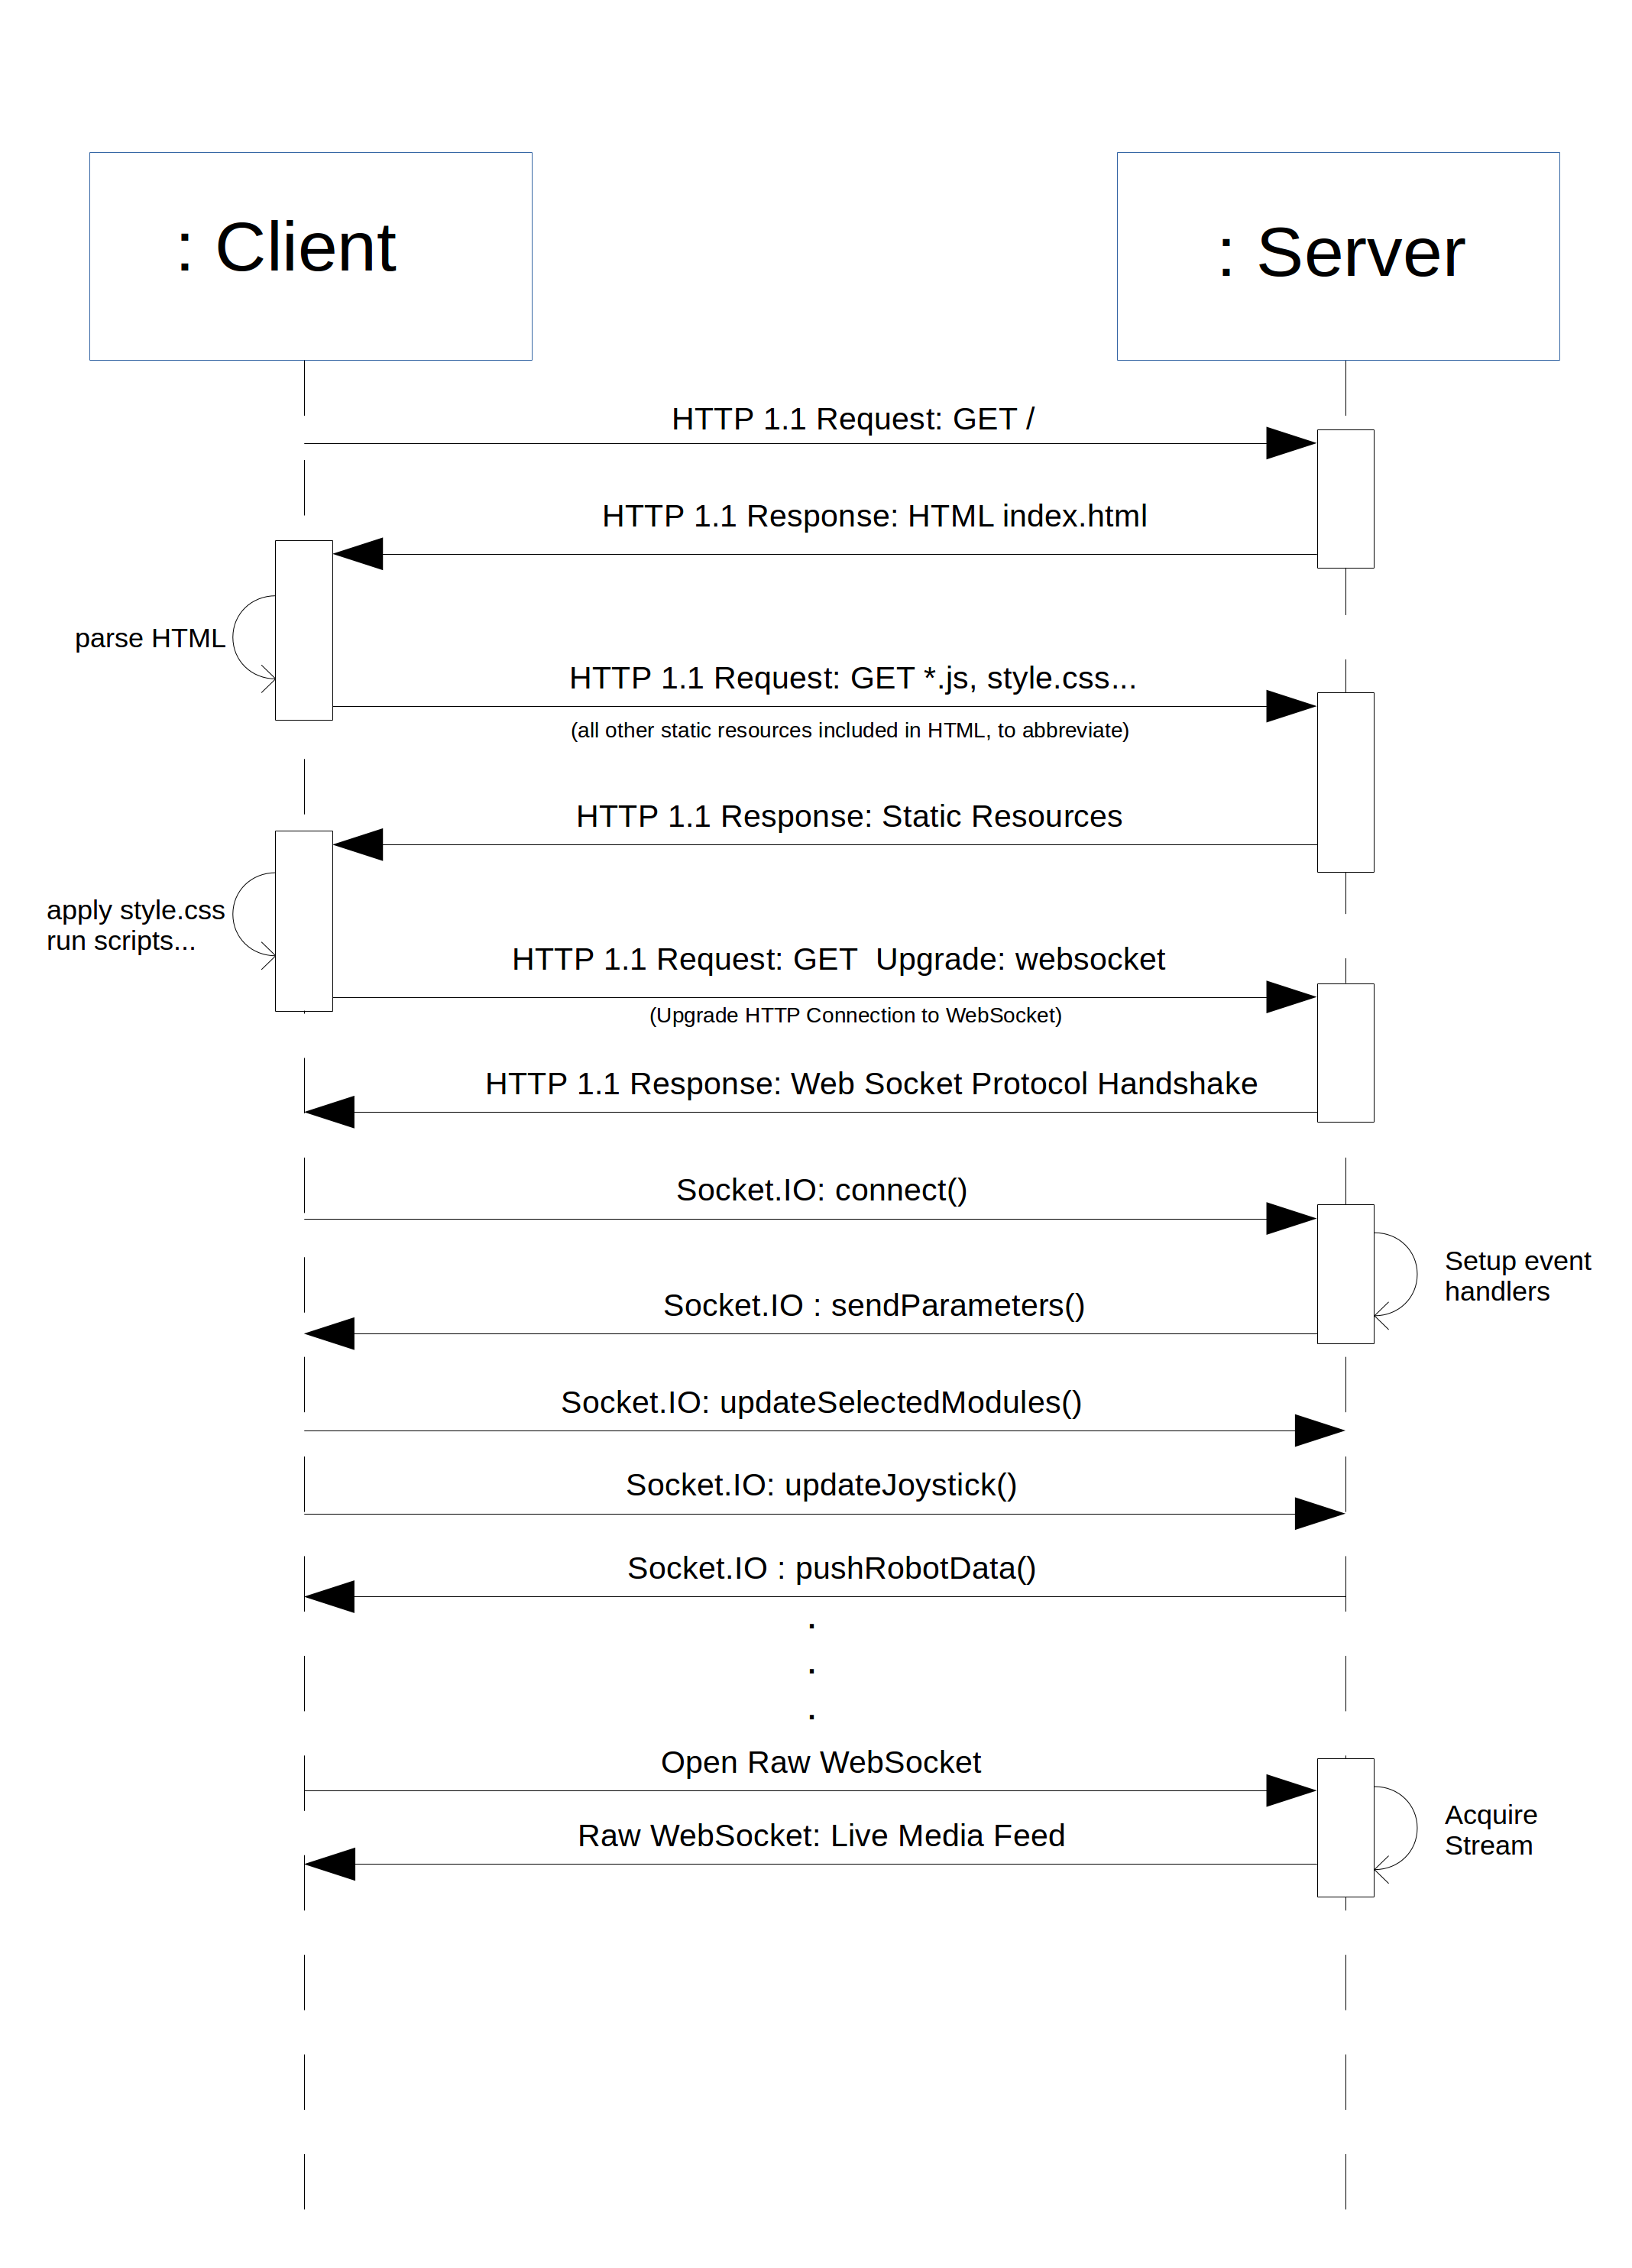
\includegraphics[width=\linewidth]{clientserverarch}
\caption{HRUI Client-Server Sequence Diagram \label{clientserverarch}}
\end{figure}
\section{Modular Front-end Architecture} \label{modularfrontendarchitecture}
\subsection{Input Modules}
\subsubsection{Joystick} \label{joystick}
\subsubsection{Gamepad} \label{gamepad}
\subsubsection{Device Orientation} \label{deviceorientation}
\subsubsection{Voice Commands} \label{voicecommands}
\subsubsection{Custom Input} \label{custominput}
\subsection{Output Modules}
\subsubsection{Data Monitor} \label{datamonitor}
\subsubsection{Live Video} \label{livevideo}
\subsubsection{Live Audio} \label{liveaudio}
\subsubsection{Geolocation}
\subsubsection{Custom Data} \label{customdata}
\subsection{Utility Modules}
\subsubsection{Script Execution} \label{scriptexecution}
\subsubsection{Profile Management} \label{profilemanagement}